Traditional logging techniques in major applications aren’t structured and many the errors logged by them don’t lead to faults, while these errors might be useful in some cases, most of the times they only decrease the readability of error logs by humans. Furthermore, there are some instances where errors, which were directly responsible for the failure of a system, were failed to be captured by these logging techniques. Considering that we are only focused on errors that lead to a failure, these techniques lead to a lot of false positives and false negatives. Here we focus only on the effective errors, or the errors which leads to the activation of faults, which in turn leads to a failure. 

A lot of work has been done previously to overcome the problems that occur by these traditional logging techniques, few of them being parsing the error logs to filter out the relevant content. While it is a great way to refine the error logs, it must go through a cumbersome work of parsing and at the same time, it does not address the core issue with error logs, which is designing a new logging mechanism. 

Most of the logging patterns try to detect errors and log it by placing a line of code at the end of a block of instructions, these techniques may not be able to detect errors such as infinite loops, etc. Therefore, instead of working on the resultant error logs, this paper aims to develop a new logging mechanism which takes care of these issues, and others such as false positives and false negatives by monitoring changes in the control flow of the program, and they do this by placing the logging instructions strategically in the code. Moreover, it aims to detect only those errors which cause failure. 


%============================================================================================================
\begin{table}[h]
	\begin{framed}
	\centering
	\resizebox{\textwidth}{!}{%
		\begin{tabular}{@{}llll@{}}
			\toprule
			Case ID & Event ID & Time             & Activity                    \\ \midrule
			1       & 85477    & 15-01-2019:14.05 & connection request received \\
			1       & 85478    & 15-01-2019:14.06 & SYN                         \\
			1       & 85479    & 15-01-2019:14.06 & SYN-ACK                     \\
			1       & 85480    & 15-01-2019:14.08 & pin verification            \\
			1       & 85481    & 15-01-2019:14.08 & verification successful     \\
			1       & 85482    & 15-01-2019:14.08 & ACK                         \\
			1       & 85483    & 15-01-2019:14.09 & connection successful       \\
			2       & 92199    & 11-02-2019:09:11 & connection request received \\
			2       & 92200    & 11-02-2019:09:12 & SYN                         \\
			2       & 92200    & 11-02-2019:09:12 & SYN-ACK                     \\
			2       & 92201    & 11-02-2019:09:13 & pin verification            \\
			2       & 92201    & 11-02-2019:09:15 & verification failed         \\
			2       & 92202    & 11-02-2019:09:16 & pin verification            \\
			2       & 92202    & 11-02-2019:09:17 & verification failed         \\
			2       & 92200    & 11-02-2019:09:18 & pin verification            \\
			2       & 92201    & 11-02-2019:09:18 & verification successful     \\
			2       & 92201    & 11-02-2019:09:20 & ACK                         \\
			2       & 92202    & 11-02-2019:09:21 & connection successful       \\ \bottomrule
		\end{tabular}%
	}
	\caption{A Sample Event Log}
	\label{table:SampleEventLog}
	\end{framed}
\end{table}
%============================================================================================================

\subsection{The Rule-Based Logging-Mechanism}

In\cite{Cinque2013}, a set of entities has been identified in a system that interacts with each other, and are prone to cause an error. This is done by referring to high-level or low-level models available at the design time, for example the architectural model, system conceptual model, or the Unified Modeling Langua. However, if these models are not available, or the logging mechanism is supposed to be implemented in an already developed system, other reverse engineering techniques can be used to isolate the entities starting from source code.

Further, a set of error-modes are established, based on the widely accepted taxonomy in the dependability area\cite{Avizienis2004}. Such as Service Error (SER: Prevents an invoked service from reaching the exit point.) Other error modes are also discussed in\cite{Cinque2013}. Different types of code injections in the form of events are then done in the source code of system which helps in the logging. These are called Login Rules (LR). Let us discuss two such Login Rules:

LR-1: Service Start (SST) and LR-2: Service End (SEN) are logged as the very first and very last instructions of a service, respectively. These login rules are made for the first error-mode, which is Service Error (SER). Note that just like LR-1 and LR-2, there are other Logging Rules (till LR-8) discussed in the paper which addresses all four errors described above. A notable Logging Rule worth mentioning is the LR-7, Heartbeat (HTB), which logs a heartbeat event periodically. 

In Rule-Based logging, these Login Rules don’t write the log-file directly but are processed dynamically by a framework called as LogBus. For example, if Service Start (SST) event is logged in LogBus, but the Service End (SEN) event fails to log within a stipulated time, it can be concluded that a Service Error (SER) has occurred. This is when LogBus updates the log file with an entry. The stipulated time, as discussed above is calculated using historical time when the system had a clean run. This is explained methodically in the paper. Methods to identify the right areas to insert these Logging Rules code is difficult, and may require usage of regular expression to parse, and later insert codes, however, the paper does not discuss any tool which can be used to insert these codes into the system automatically. Furthermore, other Login Rules like the LR-6 and LR-8 may have to be introduced into the code manually, which is a drawback. Finally, authors discuss two case studies and show that the Rule-Based logging mechanism performs drastically better than the inbuilt logging techniques in the system. Moreover, the time overhead because of introducing extra lines of logging codes are negligible.

The above logging mechanism can be extended to work within an IoT system by introducing a new entity within the system which can be in the form of a framework. Let us name it as the \textit{LogMonitor}. Contrary to traditional logging mechanisms where codes written within the system update the error logs, the LogMonitor will monitor all the events logged by the aforementioned logging rules, and eventually update the error log. This way a consistent error log can be generated for the entire system. However, this mechanism assumes that we have access to modify the internal codes of each entity within the IoT system. Other tedious methods, such as parsing of event logs\cite{he2017towards,Du2017} from each entity may have to be done, in case the internal access is unavailable.

%\subsection{Defining Error Logs}

In the previous section, an approach was discussed to make an event log consistent in an IoT system. However, there still is a need to define the event logs and categorize them in such a way that appropriate tools can be developed that works on each category efficiently. Some event logs contain time-stamps; some contain user-readable texts while others do not. Some contain just a few sets of information in the events, while some may contain hundreds of information in a single line of event log. The replication package\cite{Singh2019} contains three samples of event logs generated by various programs in the Widows Operation System. As it can be observed, event logs can range from being very complex to extremely simple. Thus, for a broad understanding, let us consider a general event log sample\cite{ProcessMiningGroupMathAndCSdepartment}, as shown in Table \ref{table:SampleEventLog}, that is readily comprehensible. The given event log can represent all possible types of event log generated by a system, as it includes some identification, a time stamp and in this case, four different attributes, viz. Activity, Award Discount, Resource and Cost. The number of attributes for an event log has no restriction. Note that just like all the entries in an event log may or may not have values for every attribute, the same has been reciprocated in the event log shown in Table \ref{table:SampleEventLog}. These event logs are bound by some underlying assumptions\cite{VanderAalst2011d}. One important assumption among the aforesaid is that each event refers to some activity. For example, in Table \ref{table:SampleEventLog}, every event consists of an activity, such as register request, check ticket, etc. A system such as the LogMonitor, as discussed in the section IIB above, could be programmed in such a way that it generates the event logs in the above format.

As can be observed, the event logs in Table \ref{table:SampleEventLog} are initially divided into Cases. Each case is further divided into Event IDs. It is worth noting that events listed under a case should only relate to precisely one case. Moreover, all the events in a case should be chronologically ordered, and at least one attribute is mandatory for an event log to exist. Issues may arise when identical events are executed in a single case. If these identical events have a corresponding termination event, it can be difficult to identify which initial event this termination event is associated with. Errors like these are categorized in \textit{Primary and Secondary Correlation Problems}\cite{VanderAalst2011d}. Also, every entry in the event log should relate to an activity. For example, in Table \ref{table:SampleEventLog}, entries refer to activities like connection request received, pin verification, verification successful, etc. In other words, the first attribute, which is \textit{activity} should definitely have a legit value for an entry in the event log to be present. The author also defines a term \textit{trace}, which is a finite sequence of unique events within a case. Furthermore, each event has been named based on its primary attribute, i.e. \textit{activity}. Therefore, the presence of this attribute has been made obligatory. In the same vein, a \textit{Simple Trace} is defined as a sequence of \textit{activities} and analogously, a \textit{Simple Event Log} is defined as a multi-set of traces. In other words, a Simple Trace has only one attribute, which is ‘activities’ in this case. That being said, any event log can be easily transformed into a simple event log by choosing one particular attribute from the set of attributes possessed by that event log. This process is particularly beneficial, if a simple approach has to be applied to a rather complex event log and can be analogized with the process of Dimensionality Reduction in machine learning.

\subsection{Process Mining}

An IoT system can be expected to generate anywhere from a thousand to hundreds of thousands of events logs instances in an hour, and as a result it is imperative to extract meaningful information from them that can help us troubleshoot any errors. Amongst many other approaches, one of them is to find possible patterns in the event logs, and then expect the IoT system to follow the pattern which was modelled. If the system deviates from the determined pattern, it can be assumed that an error has occurred and based on which part of the pattern was violated, a possible fix can be determined and automatically applied, if possible. Additionally, if the fix is determined but automatic application is not possible, for example replacement of certain parts, a repair-person can procure the replacement part in their first visit, just by accessing the event logs, thus reducing the service cost and time. 

This methodology of capturing patterns in event logs can be achieved through Process Mining. Process Mining is an excellent tool to capture meaningful information from event logs. It is mainly used to offer new medium to discover, monitor and improve processes in a quality of application domains. However, it can also be used to analyze and rectify errors in a system. It is a comparatively new research discipline that tries to extract knowledge from event logs of real processes (i.e. not assumed processes) which are readily available in today’s information systems. A report from Gartner estimated the market size of Process Mining to approach \$160 Million in 2018 \cite{Gartner2019}. This is expected to grow to \$1,421.7 million by 2023 with 50.3\% as the Compound Annual Growth Rate\cite{PressRelease2018}. The same report also predicts the growth of Process Mining usage in the IT industry (Figure \ref{fig:PMUseCase}). 

\begin{figure}[h]
	%\begin{framed}
	\centering
	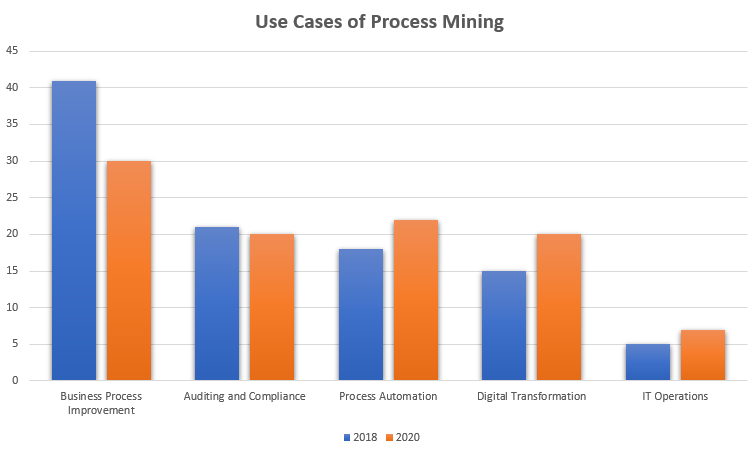
\includegraphics[width=\columnwidth]{images/use_case_process_mining.png}
	\caption{Projected Process Mining Use Case in 2020}
	\label{fig:PMUseCase}
	%\end{framed}
\end{figure}

Additionally, with the technology advancements, it has become easier to capture detailed event logs from any system, and thus, the quantity of event logs generated by any device in a period of time is increasing with every newly manufactured device. This behavior is expected, as a larger quantity of event logs implies a bigger scope to analyze the error. Thus, a robust methodology is needed to diagnose and fix the errors in an IoT system that works with event logs generated by older as well as newer systems. A process model generated by process mining using the event logs can tackle this issue. Furthermore, many commercial and academic systems have implemented process mining algorithms. The manifesto\cite{Vossen2012} also claims that an active group of researchers are working on process mining and it has become one of the “hot topics” in Business Process Management (BPM) research. Additionally, process mining functionality is added by more and more software vendors to their tools. Notable examples are: Discovery Analyst (StereoLOGIC), ARIS Process Performance Manager (Software AG), and Comprehend (Open Connect). Aforementioned reasons led us to believe that Process Mining can be an effective tool for solving the problem of Self-Healing in IoT systems. Besides this, as of July, 2015, there were 18 PhD students being funded by Philips who were working in analyzing the Philips X-Ray machines and electronic shaving devices among other items to see how these machines are used in the field, when do they fail and why do they fail, etc.\cite{Aalst2015}. Moreover, most of the X-Ray machines manufactured by Philips use Process Mining for fault diagnosis\cite{VanDerAalst2012a,Vossen2012}.

Since process mining primarily deals with event logs, it is assumed that the event logs used are in accordance with the guidelines mentioned in the section \textit{Defining Event-Logs} (vide supra). The event-log is the starting point and can be used to conduct three types of process mining. We will briefly describe these three parts below.

\textit{Process Discovery:} The most important part in Process Mining, it creates a model (called as Process Model) using event logs of real processes, but not using any theoretical or deduced information. 

\textit{Conformance Checking:} Here, a process model which was created through Process Discovery is compared with an unseen event log of the same process. This is done to check if in reality, an event log conforms to the model and vice-versa.

\textit{Enhancement:} As the word says, here the objective is to improve the existing process model using additional information recorded in the event log.

Figure \ref{fig:ProcessMiningInputOutput} describes the three types of process mining in terms of the input and output. Process Mining also covers different perspective, based on the goal that we need to achieve, these are the control-flow perspective, organizational perspective, case perspective and the time perspective. While Process Discovery still remains the most popular type of process mining, it's usage is constantly declining, where as the usage of the other two, i.e. Conformance Checking and Enhancement is increasing and is expected to increase in the future as well\ref{Gartner2019} (Figure \ref{fig:Adoption}).

\begin{figure}[h]
	%\begin{framed}
	\centering
	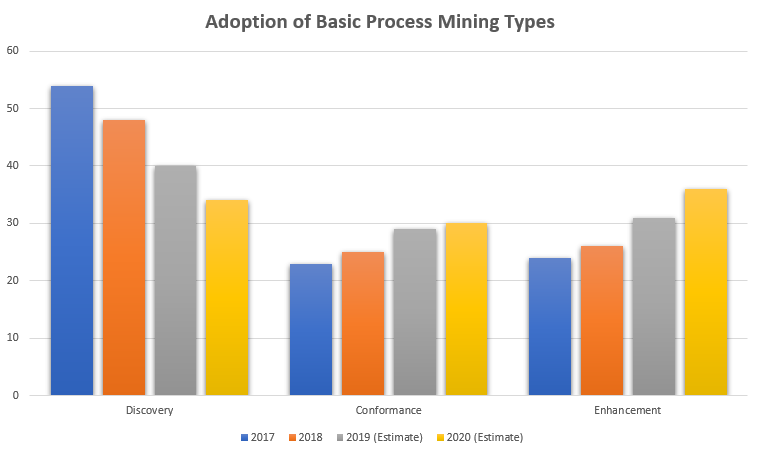
\includegraphics[width=\columnwidth]{images/adoption.png}
	\caption{Projected adoption of basic process mining types.}
	\label{fig:Adoption}
	%\end{framed}
\end{figure}

As can be seen in various machine learning algorithms, a common approach to solve a problem is by assuming an appropriate model initially (by observing the dataset) and then finding the best set of hyper-parameters; however, in Process Mining, we start from a bunch of behavior (event logs, in our case) and automatically construct the model based on the logs. This is because more often than not, there are no appropriate existing models, or the models are flawed or incomplete. Reference\cite{Rolland1998} describes process model which is \textit{roughly an anticipation of what the process will look like}. 

\begin{figure}[h]
	%\begin{framed}
	\centering
	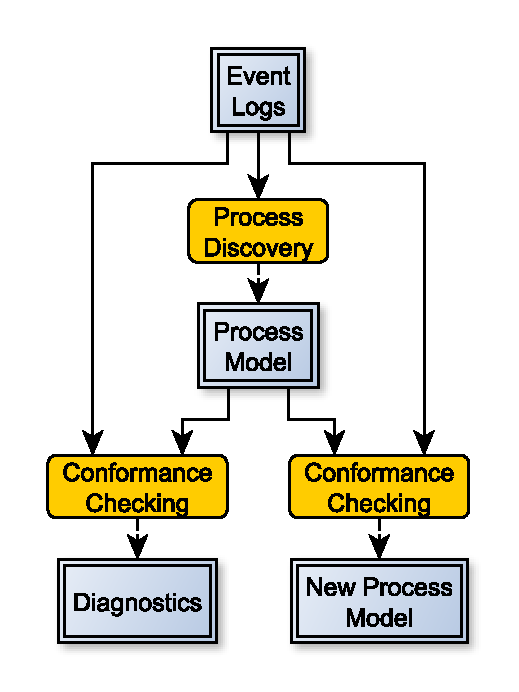
\includegraphics[width=0.6\columnwidth]{images/procesMiningInputOutput.eps}
	\caption{Different types of Process Mining in terms of Input and Output.}
	\label{fig:ProcessMiningInputOutput}
	%\end{framed}
\end{figure}

A process mining model can be represented using various notations, and the fact that there are these many notations available demonstrates the significance of process modeling. A simple event log as shown in the Figure \ref{fig:LabeledPetriNet} may be represented using an intuitive model. However, in case of an IoT system, or any electronic system whatsoever, the event logs are far more complex than the one illustrated above. As a result, a legitimate, well-defined notation should be used to represent a process model. Moreover, process models for complicated systems are prone to many problems, some of which are outlined underneath.

\begin{itemize}
	\item Oversimplification of the model: Most models have a propensity to focus only on the desirable behavior, and in a way overlook the events that are less likely to happen. There are chances that these “overlooked” events cause most of the errors and thus, the model may not be helpful.
	\item Incompetence in satisfactorily capturing human behavior: Simple and mundane process involving human engagement are prone to modifications, as human behavior is unpredictable. These changes, although minor, should nevertheless be incorporated in a model, as these nonconformities by and large result in an eventual fault.
	\item Restricted or redundant abstraction level: It is important that an appropriate abstraction level is chosen based on the objective and the input data. There is a plausibility that the model is too abstract to answer a detailed question, or conversely, a model is too detailed, and thus redundant, to answer a simple question.
\end{itemize}

A manually composed process model are susceptible to the aforementioned (and similar) problems. Moreover, a poorly designed model may engender wrong conclusions. To eradicate these problems, process mining takes the help of event logs to create a process model. An event log notifies the exact steps that the system underwent to complete any task. Additionally, using a surfeit of event logs for modelling will result in the inclusion of all the events that might be less likely to happen, as discussed above. Moreover, a process model is capable of providing different view in different abstraction levels for the same system.


\begin{figure*}
	\begin{subfigure}{.5\textwidth}
		%\begin{framed}
		\centering
		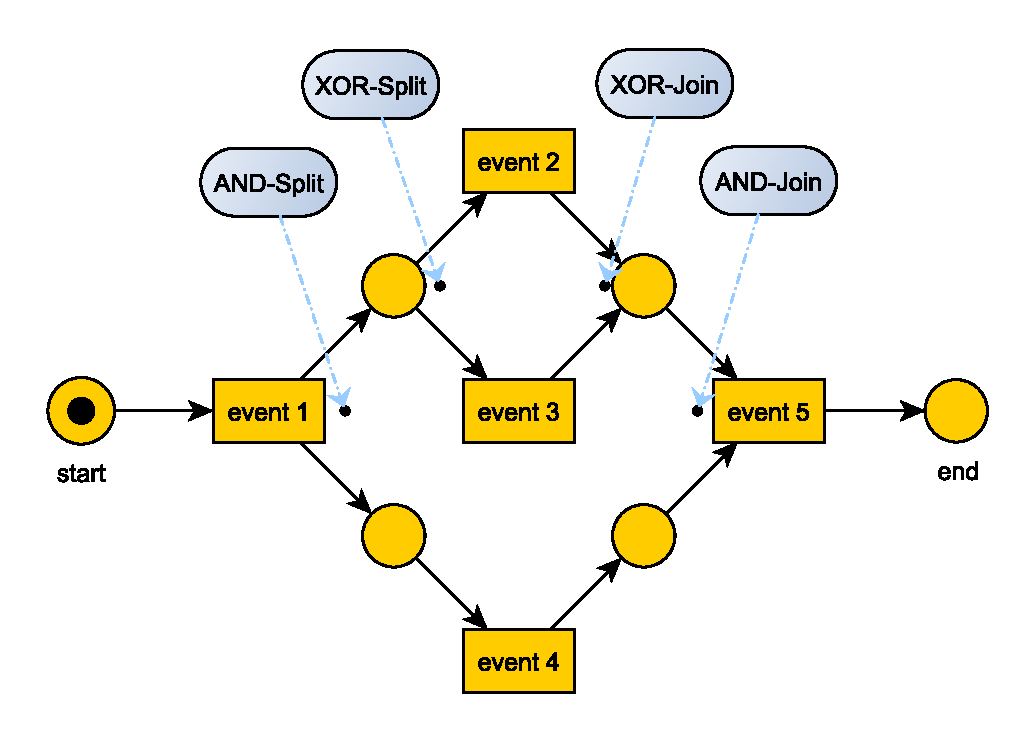
\includegraphics[width=.8\linewidth]{images/labeled-petriNet.eps}
		\caption{A Labeled Petri-Net}
		\label{fig:LabeledPetriNet}
		%\end{framed}
	\end{subfigure}%
	\begin{subfigure}{.5\textwidth}
		%\begin{framed}
		\centering
		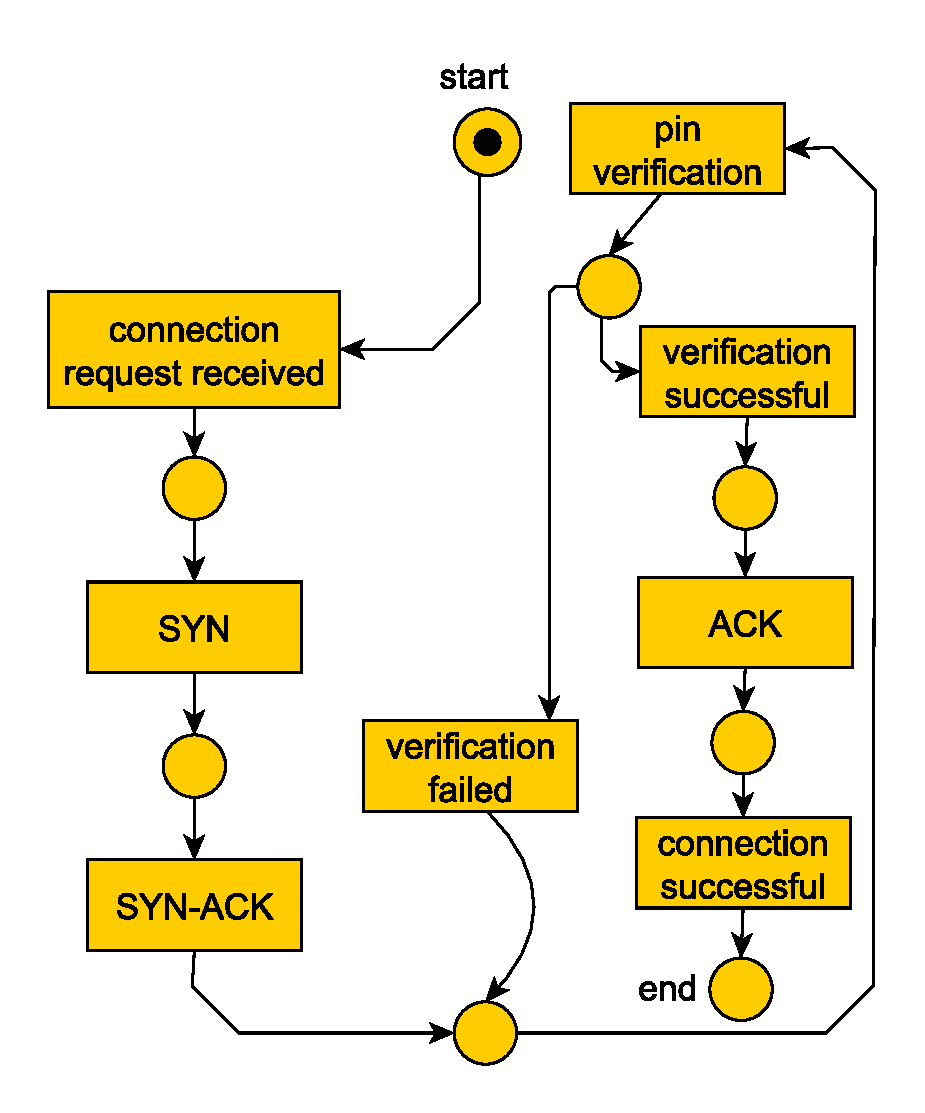
\includegraphics[width=.8\linewidth]{images/labeled-petriNetOther_update.eps}
		\caption{A petri-net process model for the sample event log displayed in Table \ref{table:SampleEventLog}}
		\label{fig:LabeledPetriNetOther}
		%\end{framed}
	\end{subfigure}
	\caption{Examples for Petri-Net Diagram}
	\label{fig:PetriNet}
\end{figure*}

Algorithms such as the α-algorithm can automatically generate process models based on event logs, as will be discussed in future sections. Notations such as EPC’s, BPMN, UML activity diagrams, etc. can be used to describe process model. It is also possible to easily convert one model to another. The primary objective of a process model is to resolve which activities need to be performed in what order. Note that activities can be executed sequentially or concurrently. They can also be optional. Furthermore, same activities can also be repeated. Let us quickly go through few of the notations that can be used to describe a process model\cite{VanderAalst2011}: 

\textit{Transition Systems}: A transition system can be considered to be the most basic process modeling notation. It consists of states and transitions. Diagrammatically, the notation resembles a non-deterministic finite automata (NFA), which can have more than one initial state and final states. The final states can also refer to as the “accept” states. The transitions, also called as “edges” in NFA denote the set of activities of the system, as described in the event log. For a path to be successfully terminated, it has to end in the final state. Moreover, if it ends at a non-final state without any ongoing transitions, it can be considered as a \textit{deadlock}. Additionally, there is also a prospect of a \textit{livelock} in case it is becomes impossible for a transition to reach the final state. A transition system can easily be translated to higher level languages such as those discussed above. However, the reverse may not be possible in some cases. These modes are simple, but they face huge issues in describing concurrent process. For example, for a process with ten parallel activities, a transition system will have to delineate more than three million execution sequences (10!), whereas a \textit{Petri-net} needs only ten transitions. Therefore, in view of the concurrent nature of process that can be observed in many IoT systems, it is imperative to use more communicative models, such as Petri-Nets for satisfactorily portraying process mining results.


\textit{Petri Nets}: As previously discussed, Petri nets are capable of describing concurrent processes without much effort like the transition systems. This is one of the oldest process modeling language. Due to its broad usage, it has also been extensively investigated; and as a result, there exists many tools to analyze them\cite{Aalst2015,VanDerAalst2012a,Vossen2012,Aalsta}. A Petri net, as suitably described by authors in\cite{Manoj2012} is “a directed bipartite graph, in which the nodes represent transitions (i.e. events that may occur, signified by bars) and places (i.e. conditions, signified by circles).” Petri nets have a static network structure. \textit{Tokens} flow through the network governed by certain firing rules. The distribution of tokens over places (also referred as \textit{marking}) determines the state of the Petri net. \cite{Petri2008} provides a broad understanding of Petri nets. Furthermore, a \textit{labeled Petri net} is an extension of the basic Petri nets, including a set of activity labels. Figure \ref{fig:LabeledPetriNet} depicts a labelled Petri-Net diagram which describes the purport of each junction. Furthermore, Figure \ref{fig:LabeledPetriNetOther} is a petri-net model for the sample event log shown in Table 2.


\textit{Workflow Nets (WF-net)}: A special type of Petri net, which is suitable for expressing workflows is used to create a process model. It is called as workflow nets\cite{VanderAalst2002}. A WF-net has a dedicated source place and sink place where the process starts and ends respectively. Another property, called soundness is defined for a WF-net. A WF-net is sound if and only if the places cannot hold multiple tokens at the same time, a proper completion is possible, there always is an option to complete and there is an absence of dead parts\cite{VanderAalst2011}.


\textit{YAWL}: The acronym stands for Yet Another Workflow Language. As the name suggests, it is a workflow modeling language. It is also an open-source workflow system. The Workflow Patterns Initiative heavily influenced its development\cite{Hofstede,VanderAalst2003}. Amongst all the open-source workflow systems, YAWL is currently the most widely used. It is similar to WF-nets that every process has a start and end condition, however activities here are called tasks. Nevertheless, just like there are places in Petri-Nets, YAWL has conditions, though tasks in this case can also be connected to each other directly, without any condition in between. It is noteworthy that YAWL also supports \textit{cancellation regions}. There may exist a cancelation region comprising of tasks, conditions and arcs. All the tokens are removed from this region after the completion of the task.


\textit{BPMN}: For modeling business processes, BPMN, or the Business Process Mining Notation has recently emerged as the most expansively used language supported by many vendors and standardized by the OMG\cite{Repa2013}.

\begin{figure*}[h]
	%\begin{framed}
	\centering
	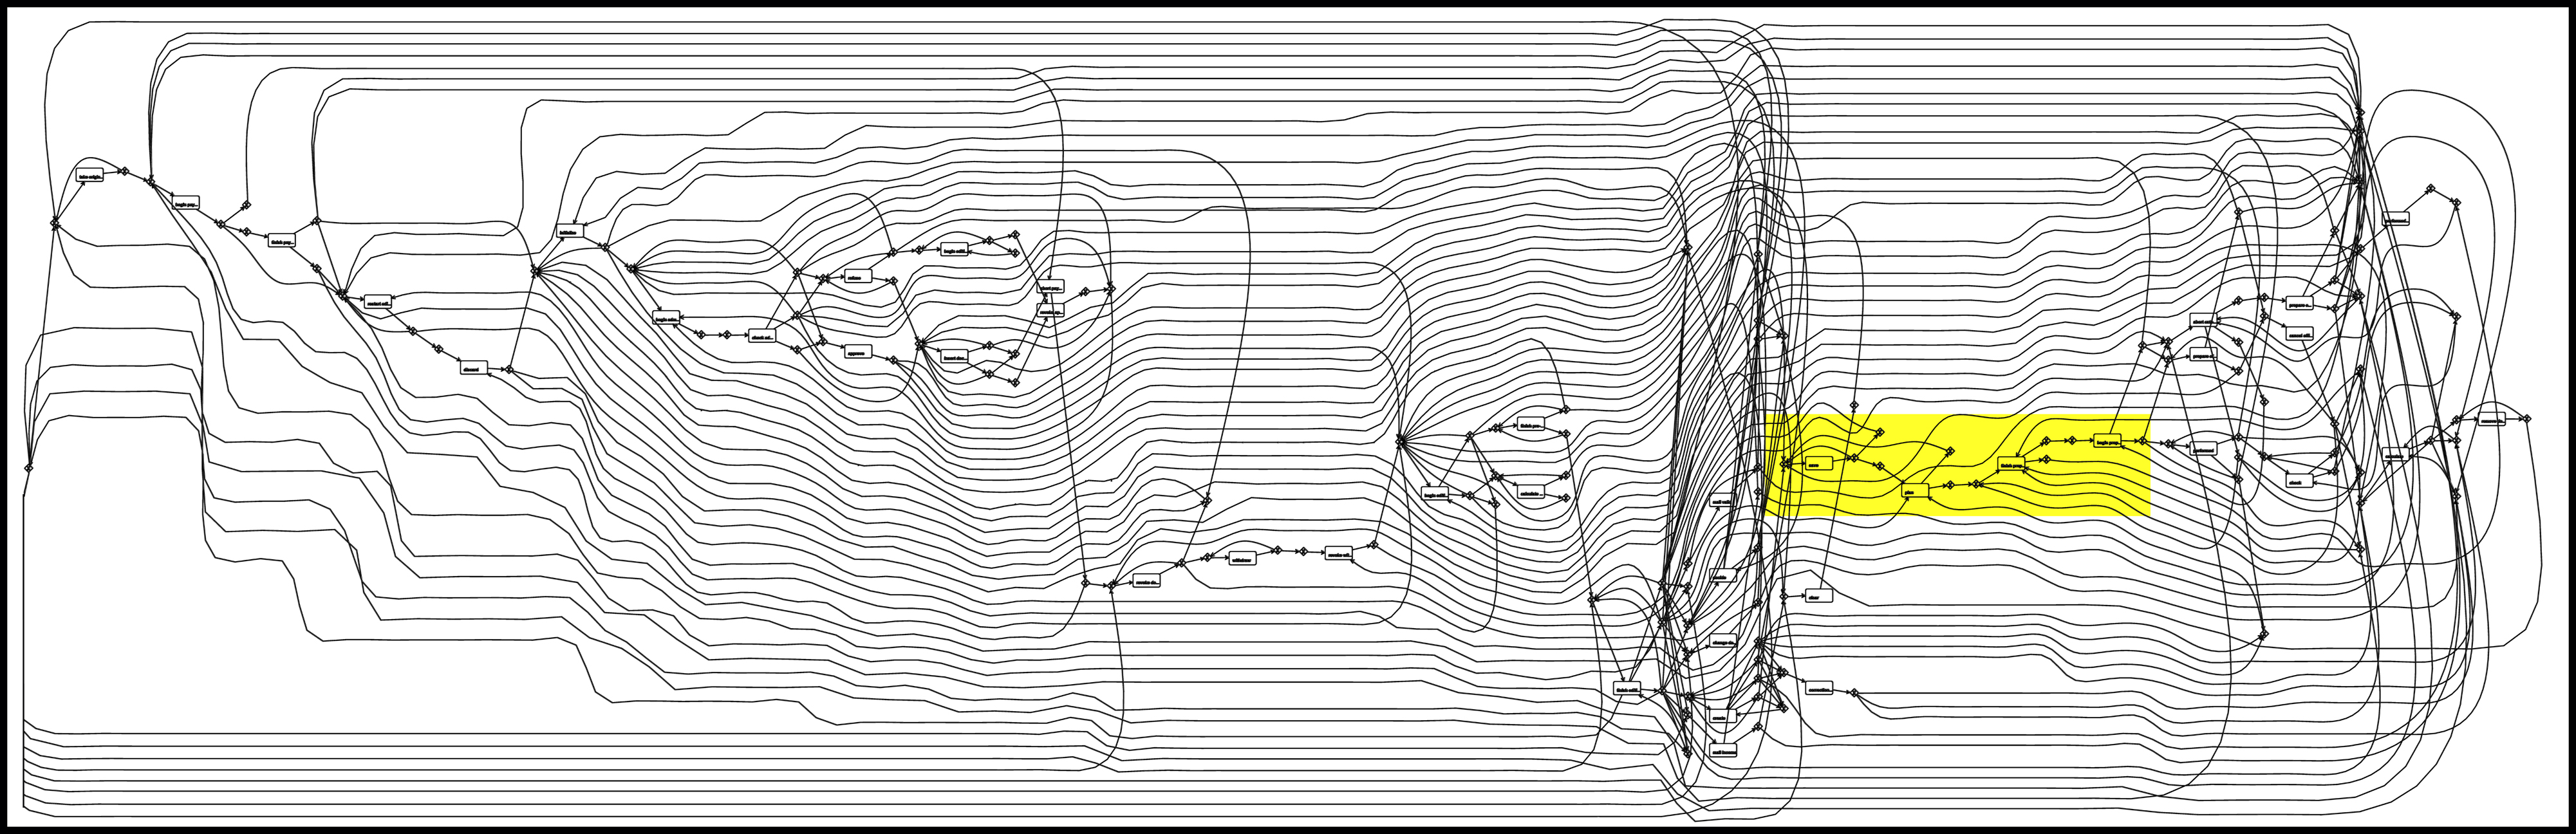
\includegraphics[width=2.2\columnwidth]{images/hiRes.jpg}
	\caption{A complex process-model using petri-nets.}
	\label{fig:HiRes}
	%\end{framed}
\end{figure*}


\begin{figure}[h]
	%\begin{framed}
	\centering
	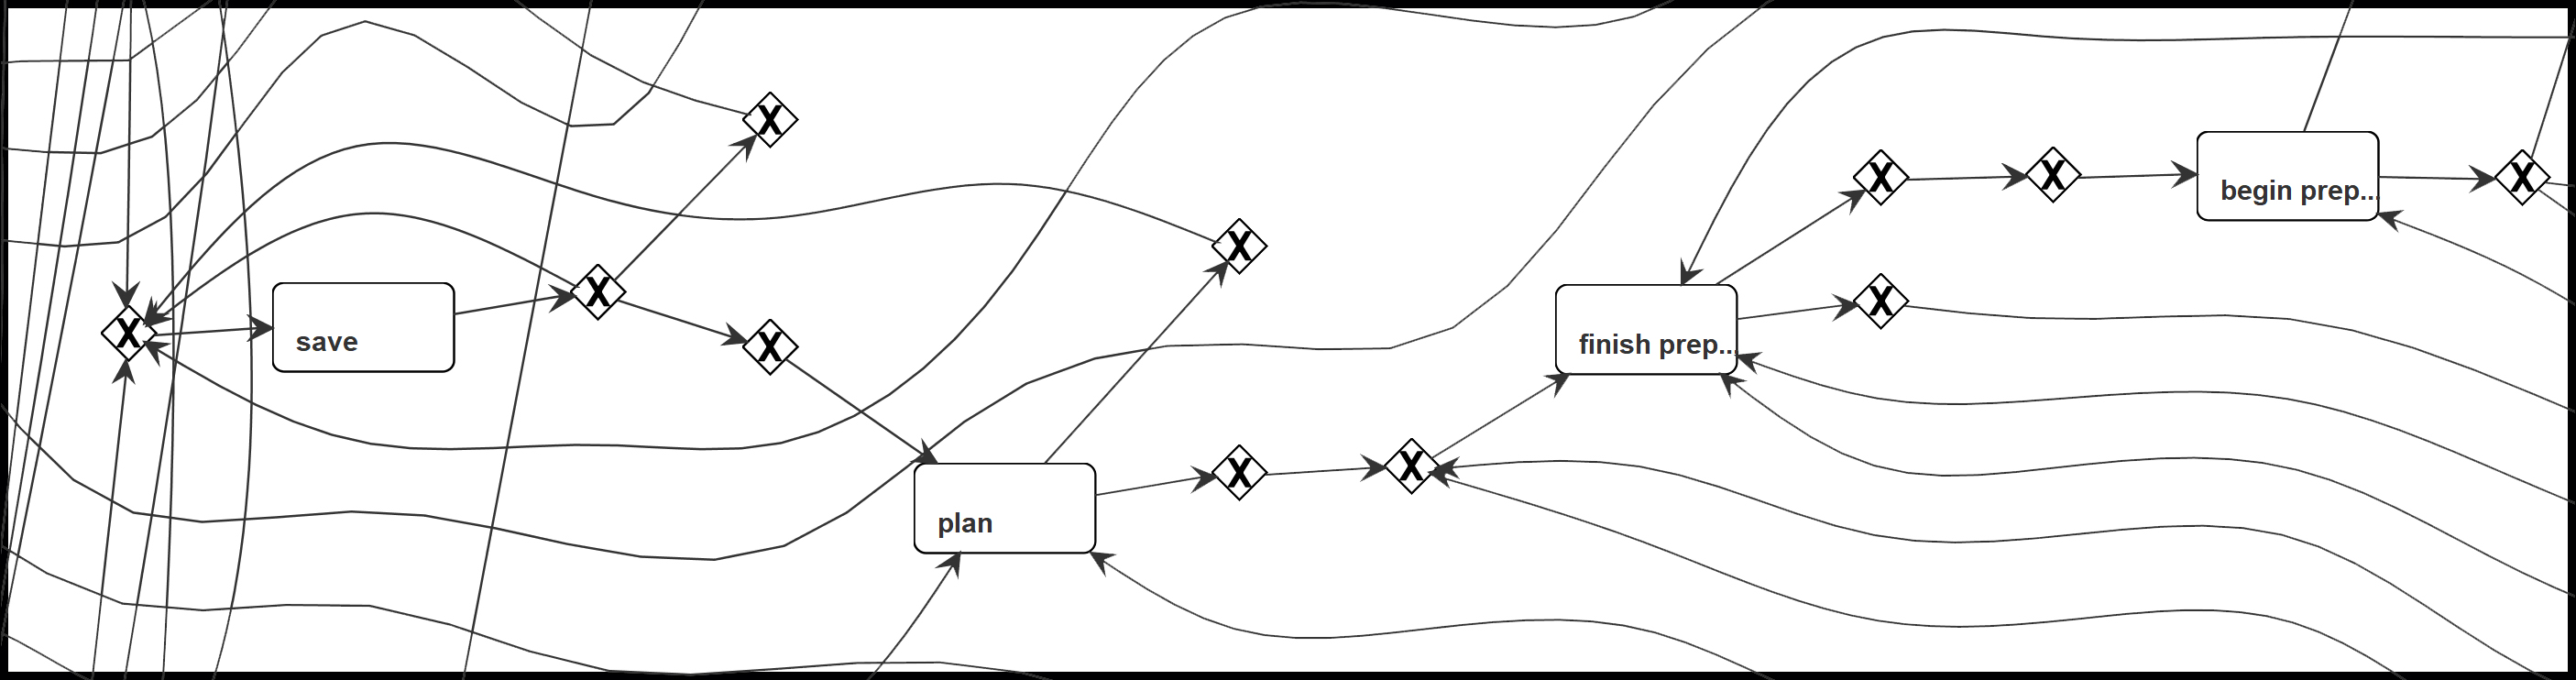
\includegraphics[width=\columnwidth]{images/hiResZoomed.jpg}
	\caption{A zoomed-in version of the shaded region showing in the Figure \ref{fig:HiRes}.}
	\label{fig:PetriNetImplementation}
	%\end{framed}
\end{figure}
 
Apart from these, other distinguished notations such as \textit{Event-Driven Process Chains (EPCs})\cite{Scheer1994} and Casual Nets are also be utilized. While EPC covers a lot of functionality provided by BPMN and YAWL, it still is only a subset of these notations as many important functionalities aren’t available in in EPC. Moreover, the semantics of EPC wasn’t clearly defined by the creators, which led to the decrease in EPC’s usage with time\cite{Mendling2006}. Note that these notations will not be elaborated upon in further sections as they are never used in the course of this survey. However, if one is more comfortable with a specific notation, note that most of the notations can be convert to the other by simple mathematical rules.


There are various existing algorithms that convert event logs to a process model as above. One of the most prominent and rather naïve algorithm is the α-algorithm\cite{VanderAalst2011a}. Additionally, Figure \ref{fig:HiRes}\footnote{This sample process model was created using the Event-Logs of BPI Challenge 2018 (https://data.4tu.nl/repository/uuid:3301445f-95e8-4ff0-98a4-901f1f204972). The log-file contains 2,514,266 instances of events that resulted in the process model as shown in the figure.}  is an example of a seemingly more complicated process model. It was created using ProM Tools. Figure \ref{fig:PetriNetImplementation} shows a zoomed-in version of the shaded region of the process model in Figure \ref{fig:HiRes}. Similarly, process models also contain detailed information, but relevant information may be available only in a particular section. 
